% LaTeX Template for Project Report, Version 2.0
% (Abstracted from a Major Project Report at CSED, NIT Calicut but can be
% modified easily to use for other reports also.)
%
% Released under Creative Commons Attribution license (CC-BY)
% Info: http://creativecommons.org/licenses/by/3.0/
%
% It is advisable to learn the basics of LaTeX before using this template.
% A good resource to start with is http://en.wikibooks.org/wiki/LaTeX/
%
% All template fields are marked with a pair of angular brackets e.g. <title here>
% except for the ones defining citation names in ref.tex.
%
% Empty space after chapter/section/subsection titles can be used to insert text.
%
% Just compile this file using pdflatex after making all required changes.

\documentclass[10pt,a4paper]{report}
\usepackage[pdftex]{graphicx} %for embedding images
\usepackage{url} %for proper url entries
\usepackage{tikz}
\usepackage{pgfplots}
\usepackage[bookmarks, colorlinks=false, pdfborder={0 0 0}, pdftitle={Assignment}, pdfauthor={Ramanathan}, pdfsubject={COMP5349 Assignment1}, pdfkeywords={<keywords here>}]{hyperref} %for creating links in the pdf version and other additional pdf attributes, no effect on the printed document
%\usepackage[final]{pdfpages} %for embedding another pdf, remove if not required
\usepackage{fullpage}
\begin{document}
\renewcommand\bibname{References} %Renames "Bibliography" to "References" on ref page

%include other pages
\begin{titlepage}

\begin{center}

% Title
\Large \textbf {COMP5349 Assignment1}\\[0.5in]
      
        \vspace{.2in}

% Submitted by
\normalsize Submitted by \\
\begin{table}[h]
\centering
\begin{tabular}{lrr}\hline \\
Student ID & Names of Students & Email\\ \\ \hline
\\
440609416 & Ramanathan Sivagurunathan & rsiv5112@uni.sydney.edu.au\\
310250811 & Woo Hyun Jung & ajun6567@uni.sydney.edu.au \\
\end{tabular}
\end{table}
\vfill

\end{center}

\end{titlepage}


\pagenumbering{roman} %numbering before main content starts
\tableofcontents

\newpage
\pagenumbering{arabic} %reset numbering to normal for the main content

\chapter{Introduction}
	This report describes the following, for each of the Hadoop Mapreduce problem given.
	
	\begin{enumerate}
	\item Design
	\item Details of Each Job
	\item Performance Characteristics
	\item Alternate Designs
	\end{enumerate}

	Our goal in the assignment was to implement a scalable, modular and efficient solution for the problem given. One of our major challenges was proliferation of map reduce jobs. With naive implementation we had several chained map reduce job but with careful use of composite keys, custom sorting, partition and grouping we could efficiently optimize out few jobs. 
	 %literature survey included in this
\chapter{Dataset}

	We have been provided with the dataset of places and photos. Some of the characteristics of the data are
	\begin{itemize}
	\item 308,133 Unique Places
	\item Size of Places file on disk is 33 MB 
	\item About 223863 Locality Places
	\item About 62363 Neighbourhood Places
	\item 80 Million Photos
	\item 700 Million Tags
	\item Size of Photos file on disk is 11 G
	\end{itemize}
	
\section{Assumptions}
	
	We have made some reasonable assumptions about the scalability. They are
	\begin{enumerate}
	\item Photos can grow significantly large. In range of Billion Photos.
	\item Tags can be significantly large. Each photo might have an average of 10 tags. 
	\end{enumerate}

	

\chapter{Task1}

	We have to find the Top 50 Locality Places (City) based on Number of Photos taken at that location. Photos taken in Neighbourhood Places within that locality has to be considered for that place itself. For each of those top 50 places we need to find the top 10 tags which has most number of photos tagged with it.
		
\section{Design}
	We have created 3 Jobs for solving the problem chained one after another \\
	\begin{itemize}
		\item [Job1:] creates counts the photos per locality  
		\item [Job2:] Sorts and Give Top 50 Locality 
		\item [Job3:] For the Top 50 Locality, Finds the top 10 tags 
	\end{itemize}

	
	\emph{Design Choice 1:}  Use of Distributed Cache \\
		Since the current number of places has about 300,000 Entries and the size is about 33 MB, we have decided to use it as a distributed cache rather than running a Mapreduce job for joining the places and photos. If each Hash entry takes about 128 Bytes (Hash, String, Value) then for a million entry it would be 128 MB. Given the RAM capacity of modern machine, this approach can scale easily upto 8 Million Entries for 1G of RAM and even more. \\
		\\
	\emph{Design Choice 2:} Reading the Photos Data Twice \\
	 	We implemented a map which reads the data and spits out two types output. One for tags and other for unique users. With that implementation the data output was about 20 Gigabytes. For the 80 Million entries for photos there we 700 million tags. Due to that we had huge amount of data which are useless causing lot of time in shuffling. And most of the data is useless as we are only concerned about top 50 locations. So we read the data again but only output tags for top 50 locations. This reduced timings massively.

	Due to these optimisations, we could get the total Running time for the problem is ~ 5 Minutes.
	
	Our design is scalable because
	\begin{enumerate}
	\item We have used Combiner everywhere to make sure less shuffling 
	\item Since we output tags only for top 50 we can scale to Petabytes still we get the best performance
	\item We use Framework to sort for better and efficient sorting	
	\end{enumerate}

\subsubsection{Job1}

\small
\begin{tabular}{| c | p{2cm} | p{2cm} | p{7cm} | }
\hline 
 Segments 
 & Input 
 & Output 
 & Pseudocode \\ \hline
 
 Mapper 
 & \scriptsize 
 1. Cache: Place.txt \newline
 2. Photos Data
 & \scriptsize 
Key: PlaceName \newline
Value: 1
 & \scriptsize 
 Setup: \newline
 1. create HashMap with (key, value) as (placeid, Placename) \newline
 2. For each line in Place.txt \newline
 		HashMap[placeid] = Placename \newline
 Map: \newline
 2. For each Text Input \newline
 		placename = HashMap(placeid)\newline
 		output(placename, 1) \newline
 \\ \hline
 
 Combiner 
 & \scriptsize
Key: PlaceName \newline
Value: 1

 & \scriptsize 
Key: PlaceName \newline
Value: List(1)
 & \scriptsize 
 Foreach  in List(1): \newline
 	 count = count + 1 \newline
 output(Placename, count) \newline
  \\ \hline
 
  Reducer 
 & \scriptsize 
Key: Place Name \newline
Value: List(count) \newline
 & \scriptsize 
Key: Place Name \newline
Value: numPhotos \newline
 & \scriptsize 
 Foreach count in List(count): \newline
 	 numPhotos = numPhotos + count \newline
 output(Placename, numPhotos) \newline
 \\ \hline
 
\end{tabular}


\subsubsection{Job2}


\small
\begin{tabular}{| c | p{3cm} | p{3cm} | p{5cm} | }
\hline 
 Segments 
 & Input 
 & Output 
 & Comments \\ \hline
 
 Mapper 
 & \scriptsize
Key: placename \newline
Value: numPhotos \newline
 & \scriptsize 
Key: numPhotos \newline
Value: Placename \newline
& \scriptsize
For Each Key, Value \newline
	output(Value, Key) \newline
 \\ \hline
 
Sorter 
& \multicolumn{2}{ |c| }{ Sort in Reverse Order }
& \scriptsize Extend Writablecomparable to reverse sort the integer and pass it to the driver. 
  \\ \hline
 
  Reducer 
 & \scriptsize 
Key: numPhotos \newline
Value: Place Name \newline
 & \scriptsize 
Key: Place Name \newline
Value:  numPhotos \newline
 & \scriptsize 
For first 50: Key and Value \newline
	Output(value, key) \newline
 \\ \hline
\end{tabular}


\subsubsection{Job3}

\bgroup
\scriptsize
\begin{tabular}{| c | p{3cm} | p{3cm} | p{5cm} | }
\hline 
 \textbf{Segments}
 & \textbf{Input}
 & \textbf{Output} 
 & \textbf{Pseudocode} \\ \hline
 
 Mapper 
 & 
 Cache1: Place.txt
 Cache2: Top 50 Places
 & 
Key: (PlaceName, Tag)
Value: 1
& 
 \textbf{Setup:} \newline
 1. create HashMap with (key, value) as (placeid, Placename) \newline
 2. For each line in Place.txt \newline
 		HashMap[placeid] = Placename \newline
\textbf{Map} \newline
1. For each Photo: \newline
	if Place is in Top 50 Places then \newline
		Output( (PlaceName, Tag), 1) \newline
 \\ \hline

 Combiner 
 & 
Key: (PlaceName, Tag)
Value: 1
 & 
Key: (PlaceName, Tag)
Value: (tagcount)
& 
 Foreach count in List(count): \newline
 	 tagcount = tagcount + count \newline
 Output( (PlaceName,Tag), tagcount) \newline
 \\ \hline 
 
 Partitioner 
&
\multicolumn{3}{ |c| }{ Partition based on Place Name} \\
  \\ \hline

  Reducer 
 & 
Key: (PlaceName, Tag)
Value: (tagcount)
 & 
 PlaceName \t numberOfPhotos \t (tag:freq)+
 & 
 \textbf{Reduce:} \newline
 For each key, List(tagcount): \newline
 	totaltagcount = totaltagcount + tagcount \newline
  If totaltagcount > one of top 10 tags for the place \newline
 	add to top 10 tags \newline
 else \newline
 	ignore tags \newline
 	
 \textbf{cleanup:} \newline
 	For each place: \newline
 		output(PlaceName \t numberOfPhotos \t (tag:freq)+) \newline

 \\ \hline
\end{tabular}
\egroup

\section{Performance}

For a highly scalable Map Reduce Job we need to make sure the following parameters are minimized
	\begin{enumerate}
	\item Time Taken for a  Map Task
	\item Time Taken for Shuffling
	\item Time Taken for a Reduce Task
	\end{enumerate}
	
	Higher the number of shuffle bytes, more the time for reduce task. So knowing where the time is more gives us better idea to optimize the solutions.	
	
	Below is our performance graph for our implementation. On X-Axis is the Input Size and on Y-Axis is Total Time taken by all mapper or Reducer. We have plotted both Mapper, Reducer, Mapper + Reducer. Due to our design the amount of work done in reducer is very minimal. 
	
	The overall running time is less than 5 Minutes, given we have enough Mapper task to run in parallel. 
	
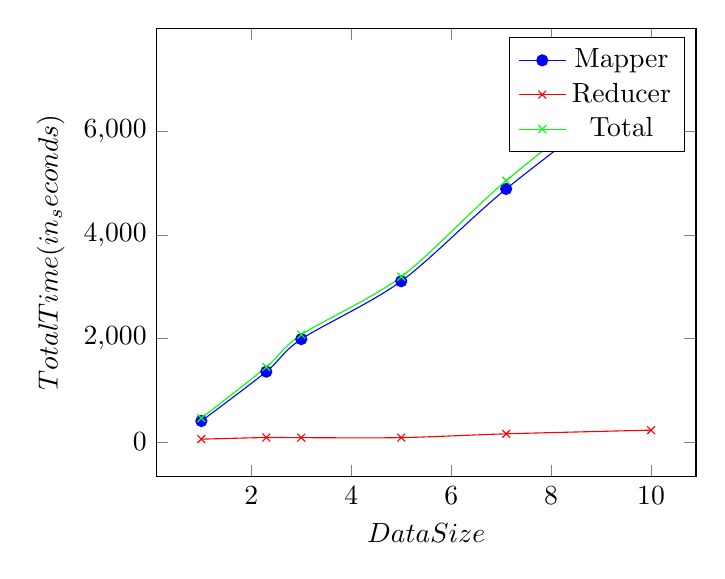
\begin{tikzpicture}
    \begin{axis}[
        xlabel=$DataSize$,
        ylabel=$TotalTime(in_seconds)$]
    \addplot[smooth,mark=*,blue] plot coordinates {
        (10, 7035)
        (7.1,4885)
        (5,3104)
        (3, 1987)
        (2.3,1359)
        (1.0, 406)
    };
    \addlegendentry{Mapper}

    \addplot[smooth,color=red,mark=x]
        plot coordinates {
            (10,230)
            (7.1,159)
            (5, 86)
            (3, 85)            
            (2.3,88)
            (1.0,56)
        };
		\addlegendentry{Reducer}
		
	    \addplot[smooth,color=green,mark=x]
        plot coordinates {
            (10,7265)
            (7.1,5044)
            (5, 3190)
            (3, 2072)            
            (2.3,1447)
            (1.0,462)
        };    
    
    	\addlegendentry{Total}
    \end{axis}
    \end{tikzpicture}
    
\chapter{Task2}

\section{Problem Definition}
	Top 10 Location for each country based on number of unique users 
	
\section{Design}
	We have created 2 Jobs for solving the problem chained one after another\\
	\begin{itemize}
		\item [Job1:] Unique Users Per Locality  
		\item [Job2:] Top 10 Location For each country
	\end{itemize}

	
	\emph{Design Choice 1:}  Use of Distributed Cache \\
		Since the current number of places has about 300,000 Entries and the size is about 33 MB, we have decided to use it as a distributed cache rather than running a Mapreduce job for joining the places and photos. If each Hash entry takes about 128 Bytes (Hash, String, Value) then for a million entry it would be 128 MB. Given the RAM capacity of modern machine, this approach can scale easily upto 8 Million Entries for 1G of RAM and even more. \\
	\emph{Design Choice 2:} Use of Composite Keys \\
		We have used composite keys for letting framework to sort and group so that we can find the unique users efficiently without the use of any hashmap which will make the solution not scalable. 
		
\subsubsection{Job1}
	This jobs outputs the unique users per locality. Each locality includes all the neighbourhood as well. Since the place.txt is small, i have used it as a distributed cache rather than adding another Map Reduce job.
	
	\textbf{Mapper} task takes the distributed cache and creates the photos and outputs a Composite key (Place, PlaceType, User) and value as (user). If the place type is Neighbourhood, there will be two outputs. One for the neighbourhood and other for the Locality. 
	
	 I have used user in key as well as value because if i sort the key based on entire key and group based on Place, i will get a sorted list of values (user). So it will be easier to find the unique as same users will be successive. So i have just traverse through the list and taking the first value. If the next is equal to previous i will skip that. 
	
	\textbf{Combiner} task is takes the key: (Place, PlaceType, User) Value: (users) and outputs only one (User). This avoids lot of bytes being shuffled across. 
	
	\textbf{Partition} is based on the Place. As we need to find the unique users per locality. This partition will allow us to find that. 
	
	\textbf{Sorting} is based on the entire key. (Place, PlaceType, User). So that the same users of the place will be successive in the resulting list. 
	
	\textbf{Grouping} is based on the place. Now we will have all the Users of the place available to reducer as sorted list. 
	
	\textbf{Reducer} task takes the (Place, PlaceType, User) as a key and list of sorted users as value. and returns (Place, PlaceType) as output key and count of unique users as Value.
	
\bgroup
\scriptsize
\begin{tabular}{| c | p{3cm} | p{3cm} | p{5cm} | }
\hline 
 \textbf{Segments}
 & \textbf{Input}
 & \textbf{Output}
 & \textbf{Comments} \\ \hline
 
 Mapper 
 & 
 Cache: Place.txt \newline
 Photos 
 & 
Key: (Place, PlaceType, User) 
Value: (user)

 & 
  \textbf{Setup:} \newline
 1. create Locality HashMap(locId, Placename) \newline
 2. create Nbrhood HashMap(nbrid, NbrhoodName) \newline
 2. For each line in Place.txt \newline
 		Locality HashMap[locId] = Placename \newline
 		Nbrhood HashMap[nbrid] = NbrhoodName \newline
 \textbf{Map:} \newline
 1. For each Line \newline
 	if PlaceType = Locality then \newline
 		Output( (PlaceName, 7, user), user)\newline
 	else if PlaceType = Nbrhood then \newline
 		Output( (PlaceName, 7, user), user) \newline
 		Output( (NbrhoodName, 22, user), user) \newline
 \\ \hline
 
 Combiner 
 & 
Key: (Place, PlaceType, User)
Value: (user)
 &  
Key: (Place, PlaceType, User)
Value: (user)
 & 
 for each key, list(value) \newline
 	Output(key, value) \newline
  \\ \hline

Partitioner
&
\multicolumn{3}{ |c| }{ Partition based on the Place } 
  \\ \hline 

Sorter
&
\multicolumn{2}{ |c| }{ Sort based on Place, PlaceType and last by User. }
& Now we have all the same users for the place consecutively. This will help us to find unique users easily.  
  \\ \hline 
  
 Grouper
&
\multicolumn{2}{ |c| }{ Group based on Place. }
& This will get all the users in the iterator, sorted. So we can count unique users easily 
  \\ \hline 
  
  Reducer 
 &
Key: (Place Name , Place Type, User)
Value: (users)
 & 
Key: (Place Name, Place Type)
Value: (unique User Count) 
& 
 for each key, list(Value) \newline
	Count the unique users in the list\newline
	Output( (PlaceName, Place Type) , Count) \newline
	\\ \hline
 \end{tabular}
\egroup

\subsubsection{Job2}

This jobs outputs the top 10 Locality for each country and for each locality a top Neighbourhood based on number of unique users. Each locality includes all the neighbourhood as well. Since the place.txt is small, i have used it as a distributed cache rather than adding another Map Reduce job.
	
	\textbf{Mapper} task takes the output of previous job with key (Place, PlaceType) and Value: (count) and returns key: (Country, Locality, Count, Name) and Value as Text with format "PlaceType:Count:Place".  Locality is in output for Neighbourhood but for actual locality the output will be "".
	
		For Example. For Locality Paris the output will be (France, "", 1000) ("7:1000:Paris")
							For Neighbourhood in Paris, the output will be (France, Paris, 100) ("22:100:Nbr1")
	
	\textbf{Partition} is based on the Country. As we need to find the Top 10 Locality per country. This partition will allow us to find that. 
	
	\textbf{Sorting} is based on the Country, Locality and reverse (count). 
	
	\textbf{Grouping} is based on the Country. Now we will have all the Descending ordered Locality for each country, followed by Neighbourhood.
	
	\textbf{Reducer} task takes the key (Country, Locality, Count, Name) and the string with format "PlaceType:Count:Place". Takes only first 10 entries for Locality. And For each Locality it takes the top Neighbourhood. 

\bgroup
\scriptsize
\begin{tabular}{| c | p{3cm} | p{3cm} | p{5cm} | }
\hline 
 \textbf{Segments}
 & \textbf{Input} 
 & \textbf{Output} 
 & \textbf{Comments} \\ \hline
 
 Mapper 
 &
 Text: placename  
 PlaceType  Count

 &  
 Key: (Country, Locality, Count, Name)
 Value: Text of Format
 "PlaceType:Count:Place"
 & 
 
 \\ \hline

 Partition 
&
\multicolumn{3}{ |c| }{ Partition based on Country } \\
  \\ \hline
 
 Sorting 
&
\multicolumn{3}{ |c| }{ Sort Country, Locality, count (descending order).  } \\
  \\ \hline

 Grouping 
&
\multicolumn{3}{ |c| }{ Grouping is based on Country } \\
  \\ \hline
 
  Reducer 
 & 
Key: (Country, Locality, Count, Name)
Value:  "PlaceType:Count:Place"
 &  
CountryName  (placeName: NumOfUsers, neighbourhoodName: NumOfUsers)+
 & 
 Gives out Top 50 Places with the number of photos count \\ \hline
\end{tabular}
\egroup

\section{Performance}
	
	For a highly scalable Map Reduce Job we need to make sure the following parameters are minimized
	\begin{enumerate}
	\item Time Taken for a  Map Task
	\item Time Taken for Shuffling
	\item Time Taken for a Reduce Task
	\end{enumerate}
	
	Higher the number of shuffle bytes, more the time for reduce task. So knowing where the time is more gives us better idea to optimize the solutions.	
	Below is our performance graph for our implementation. On X-Axis is the Input Size and on Y-Axis is Total Time taken by all mapper or Reducer. We have plotted both Mapper, Reducer, Mapper + Reducer. Due to our design the amount of work done in reducer is very minimal. \\
	\\
	The overall running time is less than 3 Minutes, given we have enough Mapper task to run in parallel. 
	
	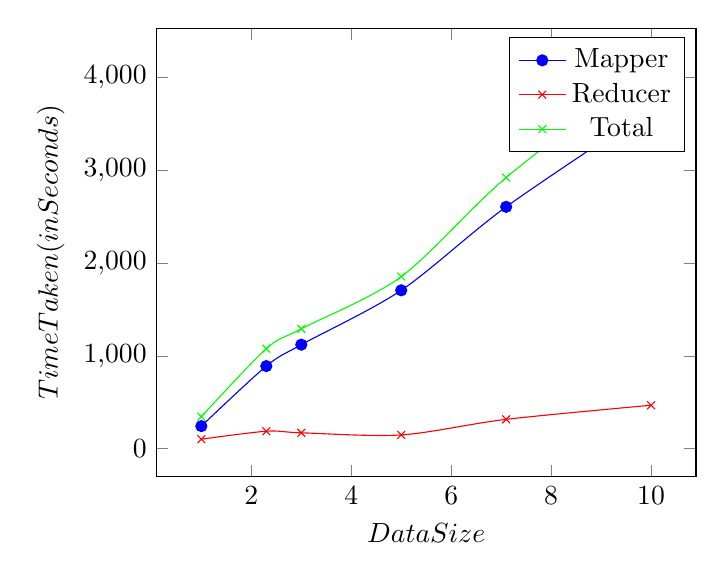
\begin{tikzpicture}
    \begin{axis}[
        xlabel=$DataSize$,
        ylabel=$TimeTaken(inSeconds)$]
    \addplot[smooth,mark=*,blue] plot coordinates {
        (10,3662)
        (7.1,2607)
        (5,1707)
        (3, 1121)
        (2.3,890)
        (1.0, 243)
    };
    \addlegendentry{Mapper}

    \addplot[smooth,color=red,mark=x]
        plot coordinates {
            (10,468)
            (7.1,316)
            (5,148)
            (3,171)            
            (2.3,188)
            (1.0,102)
        };
    \addlegendentry{Reducer}
    
    \addplot[smooth,color=green,mark=x]
        plot coordinates {
            (10,4130)
            (7.1,2923)
            (5, 1855)
            (3,1292)            
            (2.3,1078)
            (1.0,345)
        };
    \addlegendentry{Total}    
    
    \end{axis}
    \end{tikzpicture}
    
   \section{Alternate Design}
   		It is possible to design a solution for the given problem with just one Map Reduce Job. Implementation for the design is also provided. 
   		
   		Since the number of places is small, we are using the places in the distributed cache. \newline
\bgroup
\scriptsize
\begin{tabular}{| c | p{3cm} | p{3cm} | p{5cm} | }
\hline 
 Segments 
 & Input 
 & Output 
 & Comments \\ \hline
 
 Mapper 
 & \scriptsize 
 Text: Photos

 & \scriptsize 
 Key: (Country, Locality, Neighbourhood, User)
 Value: 1
 & For each Neighbourhood there are two output one for (Country, Locality, "", User) and (Country, Locality, Nbrhood, User)
 \\ \hline

 Combiner 
 & \scriptsize 
 Key: (Country, Locality, Neighbourhood, User)
 Value: 1

 & \scriptsize 
 Key: (Country, Locality, Neighbourhood, User)
 Value: 1
 & For every key we just output only one entry. This is for counting unique users.
 \\ \hline

 Partition 
&
\multicolumn{3}{ |c| }{ Partition based on Country } \\
  \\ \hline
  Reducer 
 & \scriptsize 
Key: (Country, Locality, Count, Name)
Value:  1
 & \scriptsize 
CountryName \t (placeName: NumOfUsers, neighbourhoodName: NumOfUsers)+
 & \scriptsize 
 We have a hash map of all the places per country. So for every entry we use hashmap to count and at the end of the Reducer (In Cleanup Function) we output the desired output taken from the hashmap.  \\ \hline
\end{tabular}
\egroup
\subsection{Pros and Cons}

Pros:
\begin{enumerate}
	\item Number of Map Reduce Job is reduced
	\item Better Performance if we have small sized data.
\end{enumerate}

Cons:
\begin{enumerate}
	\item Not scalable as few countries will have more places and more photos will be there. So a single reducer will be highly overloaded causing the delay
\end{enumerate}
\cleardoublepage
%\pagebreak
\phantomsection
\addcontentsline{toc}{chapter}{References}
\begin{thebibliography}{99}

\bibitem{hadoop}Hadoop Map Reduce Framework\ \url{http://hadoop.apache.org}

\end{thebibliography}

\end{document}
